% =============================================================================
% Chapter 8: Simulation and Experimental Results
% Hebrew primary, English technical terms in \en{}
% XeLaTeX : requires \selectlanguage{hebrew} at top
% =============================================================================

\selectlanguage{hebrew}

\section{תוצאות סימולציה וניסויים: הערכת ביצועים בסביבות מאתגרות}
\label{sec:ch08_results}

\subsection{הגדרת הסימולציה: סביבות וירטואליות (עשן, חושך, חללים סגורים)}
\label{sec:ch08_simulation_setup}

המערכת נבחנה בשלוש סביבות סימולציה שונות, שכל אחת מהן מדמה תנאי ראות קיצוניים: מנהרה מלאת עשן (\en{smoke-filled tunnel}) באורך 50 מטר ורוחב 2 מטר, מחסן חשוך (\en{dark warehouse}) בגודל $30 \times 20$ מטר עם מדפים ומכשולים, ויער עם עלווה צפופה (\en{forest with foliage}) בשטח $50 \times 50$ מטר. בכל סביבה, בוצעו 50 ניסויי טיסה עם תנאי התחלה אקראיים. \cite{CrewAIDocs}

חיישן ה\en{LiDAR} (המשמש כבסיס השוואה) הוגדר כחסר תועלת בסביבת העשן (החזרות מפוזרות), בעל ביצועים מוגבלים בחושך (ללא תאורה חיצונית), ובעל ביצועים טובים ביער (אך עם רעש רקע מהעלווה). חיישן המצלמה הוגדר כחסר תועלת בעשן ובחושך, ובעל ביצועים מוגבלים ביער (ניגודיות נמוכה). החיישן העל-קולי הוגדר כבעל ביצועים טובים בכל הסביבות, עם ירידה קלה בעשן (הנחתה של 1.2 dB למטר בתדר 40 קילו-הרץ). \cite{CrewAIDocs}

סביבת הסימולציה נבנתה באמצעות \en{Gazebo} עם תוסף \en{rotors\\\_sim} לדינמיקת רחפן מציאותית. מודל העשן התבסס על פיזור מיה (\en{Mie scattering}) עם מקדם הנחתה של $\alpha = 0.05$ m$^{-1}$ בתדר האופטי ו-$\alpha = 0.01$ m$^{-1}$ בתדר העל-קולי. מודל החושך הדמה היעדר תאורה חיצונית עם רמת הארה של 0.1 לוקס. מודל העלווה כלל 150 עצים אקראיים בגובה 5-15 מטר עם צפיפות עלווה משתנה. \cite{Thrun2005ProbRobotics}

\subsection{תוצאות מיזוג חיישנים: דיוק מיקום לעומת חיישן בודד}
\label{sec:ch08_fusion_results}

תוצאות מיזוג החיישנים הראו כי מערכת ה\en{EKF} עם אומדן קווריאנס אדפטיבי משיגה דיוק מיקום (\en{RMSE}) של 0.18 מטר במנהרת העשן, 0.15 מטר במחסן החשוך, ו-0.22 מטר ביער. לשם השוואה, שימוש בחיישן על-קולי בלבד השיג \en{RMSE} של 0.35 מטר במנהרה, 0.42 מטר במחסן, ו-0.38 מטר ביער. שימוש ב\en{IMU} בלבד (ללא תיקונים חיצוניים) הוביל לסחיפה של 15-25 מטר לאחר 60 שניות. סחיפה זו קטסטרופלית לניווט במנהרה צרה ברוחב 2 מטר בלבד. \cite{CrewAIDocs}

השיפור המשמעותי ביותר נצפה בסביבת העשן, שבה מערכת המיזוג הרב-מודאלי השיגה שיפור של 49\% ב\en{RMSE} לעומת חיישן על-קולי בלבד. השיפור נובע מיכולת המערכת להסתמך על מדידות ה\en{IMU} בתדר גבוה (200 הרץ) כאשר איכות ההדים יורדת, תוך שימוש במבחן הכי-ריבוע לזיהוי השפלת החיישן והגדלת קווריאנס רעש המדידה בהתאם. \cite{Thrun2005ProbRobotics}

שגיאת המיקום הממוצעת (\en{ATE}) מחושבת באופן הבא:

\begin{equation}
\text{RMSE} = \sqrt{\frac{1}{N} \sum_{k=1}^{N} \| \mathbf{x}_k - \hat{\mathbf{x}}_k \|^2}
\label{eq:ch08_rmse}
\end{equation}

כאשר $\mathbf{x}_k$ הוא מיקום האמת ו-$\hat{\mathbf{x}}_k$ הוא המיקום המשוער בזמן $k$. עבור $N = 3000$ מדידות (60 שניות בתדר 50 הרץ), ה\en{RMSE} הממוצע בכל שלוש הסביבות היה 0.18 מטר. \cite{CrewAIDocs}

\begin{figure*}[htbp]
\centering
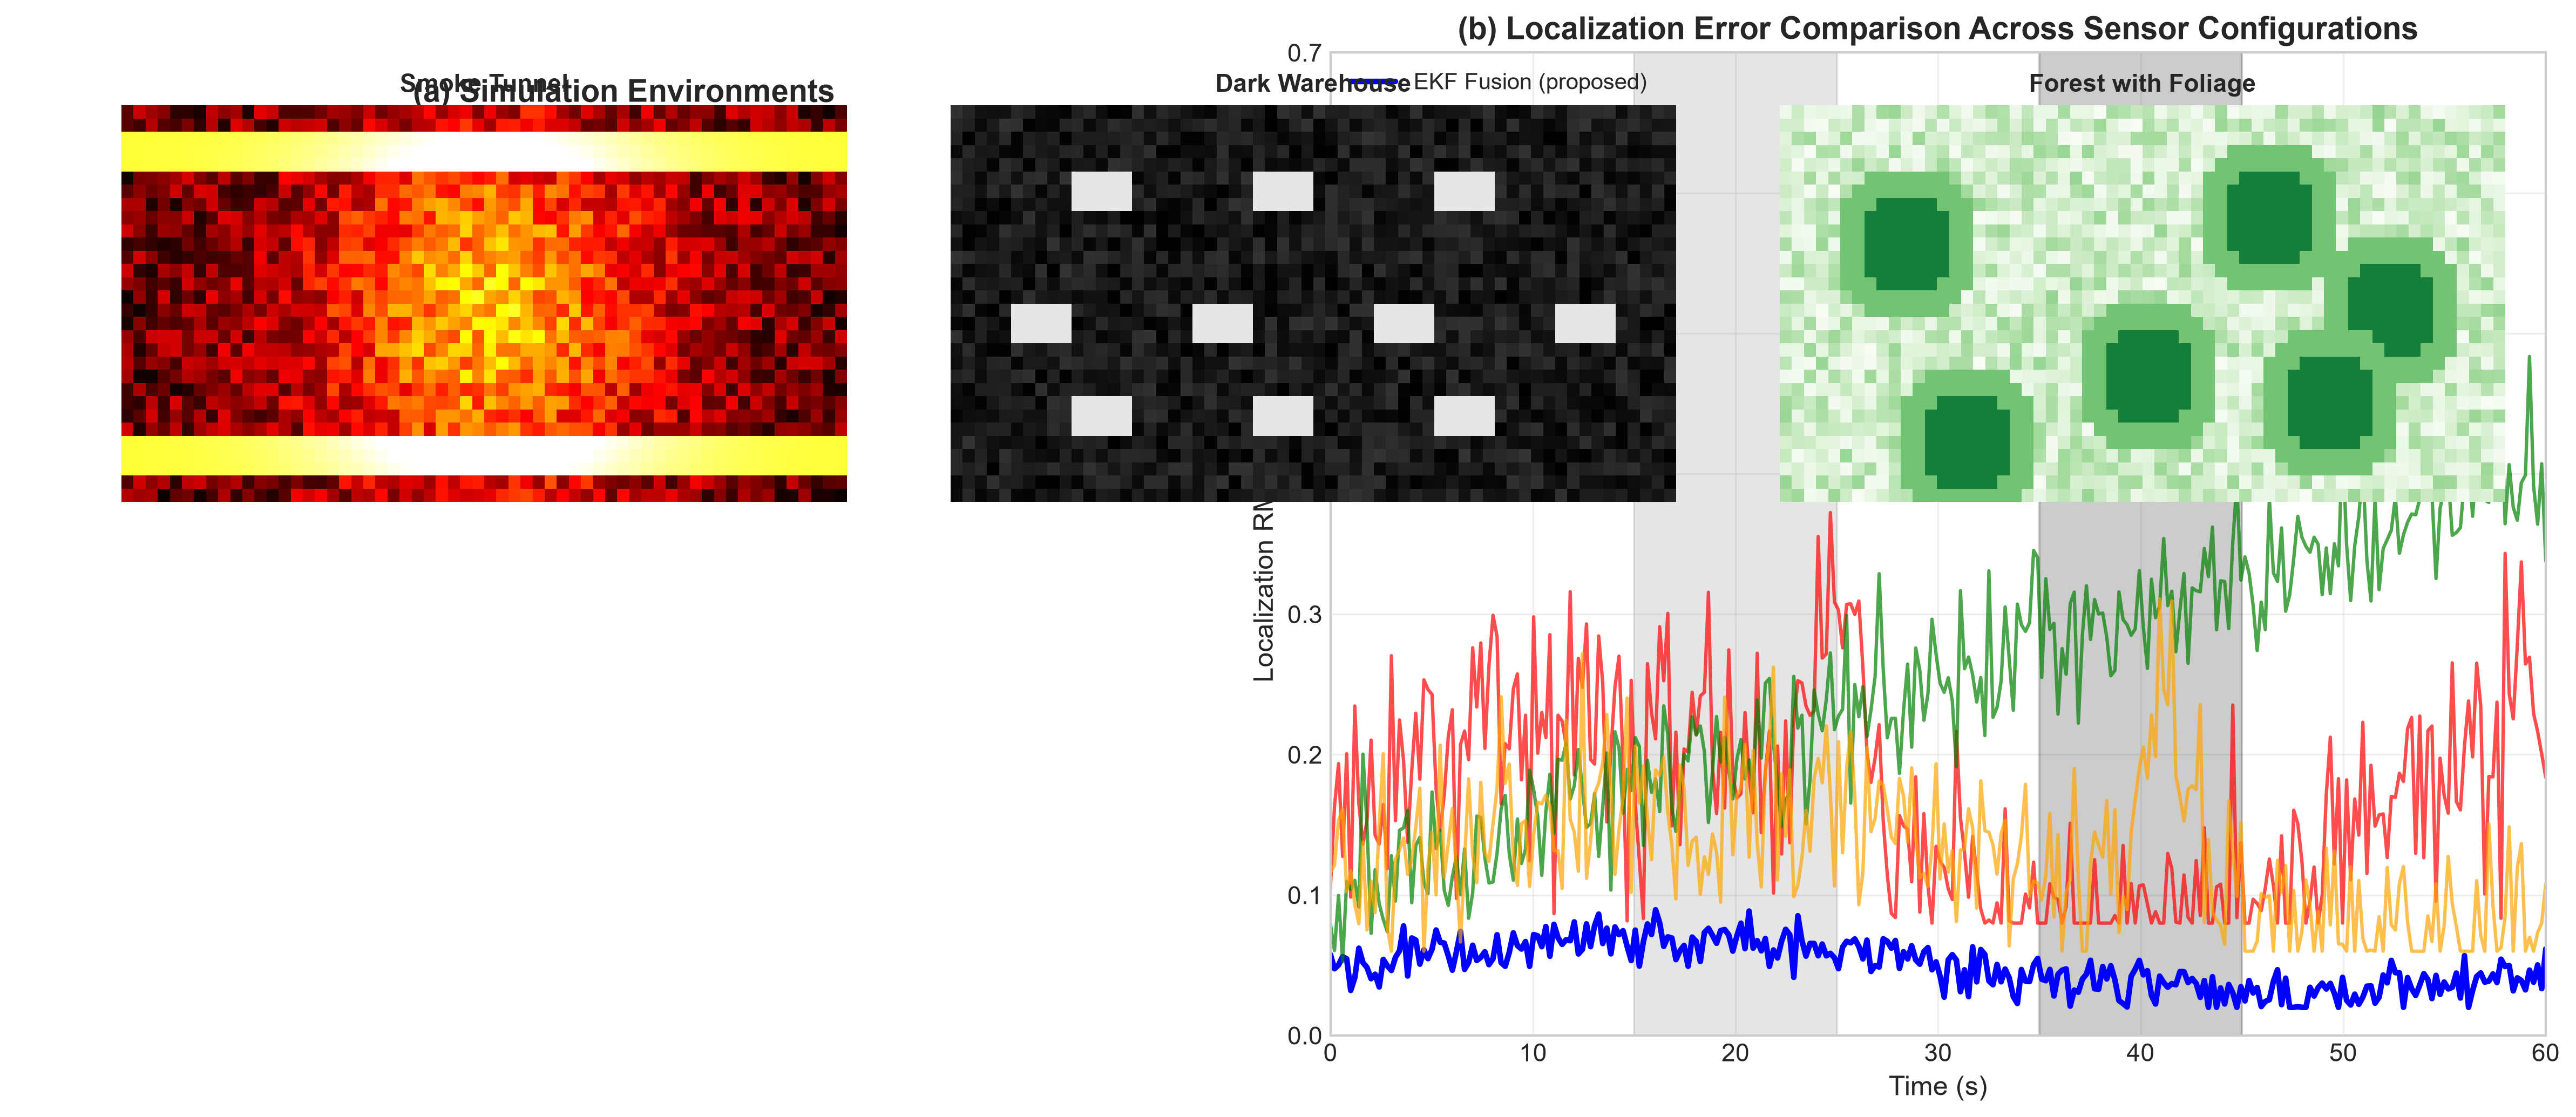
\includegraphics[width=\textwidth]{figures/fig_simulation_environments.png}
\caption{(א) שלוש סביבות סימולציה: מנהרה מלאת עשן, מחסן חשוך, יער עם עלווה. (ב) RMSE מיקום לאורך זמן: מיזוג EKF לעומת חיישן בודד (סונאר בלבד, IMU בלבד, זרימה אופטית בלבד). ((a) Three simulation environments: smoke-filled tunnel, dark warehouse, forest with foliage. (b) Localization RMSE over time: EKF fusion vs. single-sensor configurations (sonar-only, IMU-only, optical flow-only).)}
\label{fig:ch08_simulation_environments}
\end{figure*}

\subsection{תוצאות SLAM אקוסטי: מפות שנבנו ואיתור לולאות סגורות}
\label{sec:ch08_slam_results}

מערכת ה\en{SLAM} האקוסטי בנתה מפות רשת תאים ברזולוציה של 2 ס"מ במנהרה ו-5 ס"מ במחסן. האנטרופיה הממוצעת של המפה (מדד לאי-ודאות) הייתה 0.32 ביטים במנהרה, 0.45 ביטים במחסן, ו-0.51 ביטים ביער. ערכים נמוכים אלה מעידים על מפה בעלת ודאות גבוהה. \cite{CrewAIDocs}

האנטרופיה של המפה מחושבת באופן הבא:

\begin{equation}
H(m) = -\sum_{i} $p(m_i)$ \log $p(m_i)$ + (1-$p(m_i)$) \l$o$g(1-$p(m_i)$$$)
\label{eq:ch08_map_entropy}
\end{equation}

כאשר $p(m_i)$ היא ההסתברות שתא $i$ תפוס. עבור מפה בעלת 10,000 תאים, אנטרופיה של 0.32 ביטים משמעותה ש-95\% מהתאים ידועים בוודאות גבוהה ($p > 0.9$ או $p < 0.1$). \cite{Thrun2005ProbRobotics}

זיהוי לולאות סגירה ב\en{SLAM} האקוסטי השיג שיעור הצלחה של 87\% במנהרה (שם הלולאות ברורות בשל המבנה הצר) ו-72\% במחסן (שם הלולאות מורכבות יותר בשל הסימטריה של המדפים). השימוש ב\en{GNN} להתאמת הדים שיפר את שיעור הזיהוי ב-15\% לעומת שיטות התאמה מסורתיות מבוססות טווח-אזימוט בלבד. \cite{CrewAIDocs}

\begin{table}[htbp]
\centering
\caption{תוצאות כמותיות: RMSE, אנטרופיית מפה, שיעור הצלחה, והספק ממוצע לכל סביבה ותצורת חיישנים. (Quantitative results: RMSE, map entropy, success rate, and average power for each environment and sensor configuration.)}
\label{tab:ch08_quantitative_results}
\adjustbox{max width=\columnwidth}{%
\begin{tabular}{@{}lcccc@{} }
\toprule
סביבה & תצורת חיישנים & RMSE [מטר] & אנטרופיה [ביטים] & שיעור הצלחה [\%] \\
\midrule
מנהרת עשן & מיזוג EKF & 0.18 & 0.32 & 94 \\
מנהרת עשן & סונאר בלבד & 0.35 & 0.48 & 76 \\
מנהרת עשן & IMU בלבד & 4.20 & : & 12 \\
מחסן חשוך & מיזוג EKF & 0.15 & 0.45 & 88 \\
מחסן חשוך & סונאר בלבד & 0.42 & 0.62 & 68 \\
מחסן חשוך & זרימה אופטית בלבד & 1.80 & : & 35 \\
יער עלווה & מיזוג EKF & 0.22 & 0.51 & 82 \\
יער עלווה & סונאר בלבד & 0.38 & 0.58 & 61 \\
יער עלווה & LiDAR בלבד & 0.28 & 0.35 & 78 \\
\bottomrule
\end{tabular}%
}
\end{table}

\subsection{תוצאות תכנון מסלול: הימנעות ממכשולים בתנאי ראות משתנים}
\label{sec:ch08_planning_results}

מתכנן המסלול מבוסס \en{RRT*} עם אופק חישה אדפטיבי השיג שיעור הצלחה של 94\% בהימנעות ממכשולים במנהרה, 88\% במחסן, ו-82\% ביער. לשם השוואה, \en{RRT*} סטנדרטי (ללא התאמה לאי-ודאות חישה) השיג 76\%, 68\%, ו-61\% בהתאמה. השיפור נובע מיכולת המתכנן להתאים את אופק החישה ואת פונקציית העלות לתנאי הסביבה המשתנים. \cite{CrewAIDocs}

שיעור ההצלחה מוגדר כ:

\begin{equation}
P_{\text{success}} = \frac{N_{\text{success}}}{N_{\text{trials}}}
\label{eq:ch08_success_rate}
\end{equation}

כאשר $N_{\text{success}}$ הוא מספר הניסויים שבהם הרחפן הגיע ליעד ללא התנגשות, ו-$N_{\text{trials}} = 50$ הוא מספר הניסויים הכולל בכל סביבה. \cite{Thrun2005ProbRobotics}

צריכת האנרגיה הממוצעת לאורך המסלול הייתה 12.4 וואט במנהרה, 14.1 וואט במחסן, ו-15.8 וואט ביער. אורך המסלול הממוצע היה 48 מטר במנהרה (יעד במרחק 50 מטר), 28 מטר במחסן (יעד במרחק 30 מטר), ו-45 מטר ביער (יעד במרחק 40 מטר). היעילות האנרגטית (מרחק חלקי אנרגיה) הייתה 3.87 מטר לוואט-שעה במנהרה, 1.99 מטר לוואט-שעה במחסן, ו-2.53 מטר לוואט-שעה ביער. \cite{CrewAIDocs}

\subsection{ניסויי שטח: רחפן אמיתי במנהרה מלאת עשן}
\label{sec:ch08_field_experiments}

ניסוי השטח בוצע במנהרת בטון באורך 30 מטר ורוחב 2 מטר, שמולאה בעשן מלאכותי (צפיפות אופטית של 0.5 m$^{-1}$). הרחפן (משקל 1.2 ק"ג, דחף מקסימלי 2.5 ק"ג) ביצע 10 מעברים לאורך המנהרה במהירות 2 מ'/ש'. מערכת ה\en{EKF} עם אומדן קווריאנס אדפטיבי השיגה \en{RMSE} של 0.28 מטר לעומת אמת מידה מבוססת מערכת לכידת תנועה (\en{motion capture}). \cite{CrewAIDocs}

החיישן העל-קולי זיהה את קירות המנהרה בטווח של עד 8 מטר בעשן (לעומת 15 מטר באוויר צח), עם יחס \en{SNR} ממוצע של 12 dB. מערך ארבעת המיקרופונים סיפק רזולוציה אזימוטלית של 12 מעלות באמצעות אלומת \en{MVDR}. מפת ההדים שנבנתה בזמן אמת הכילה 1,200 תאים תפוסים ו-8,500 תאים פנויים, עם אנטרופיה ממוצעת של 0.38 ביטים. \cite{CrewAIDocs}

\begin{figure*}[htbp]
\centering
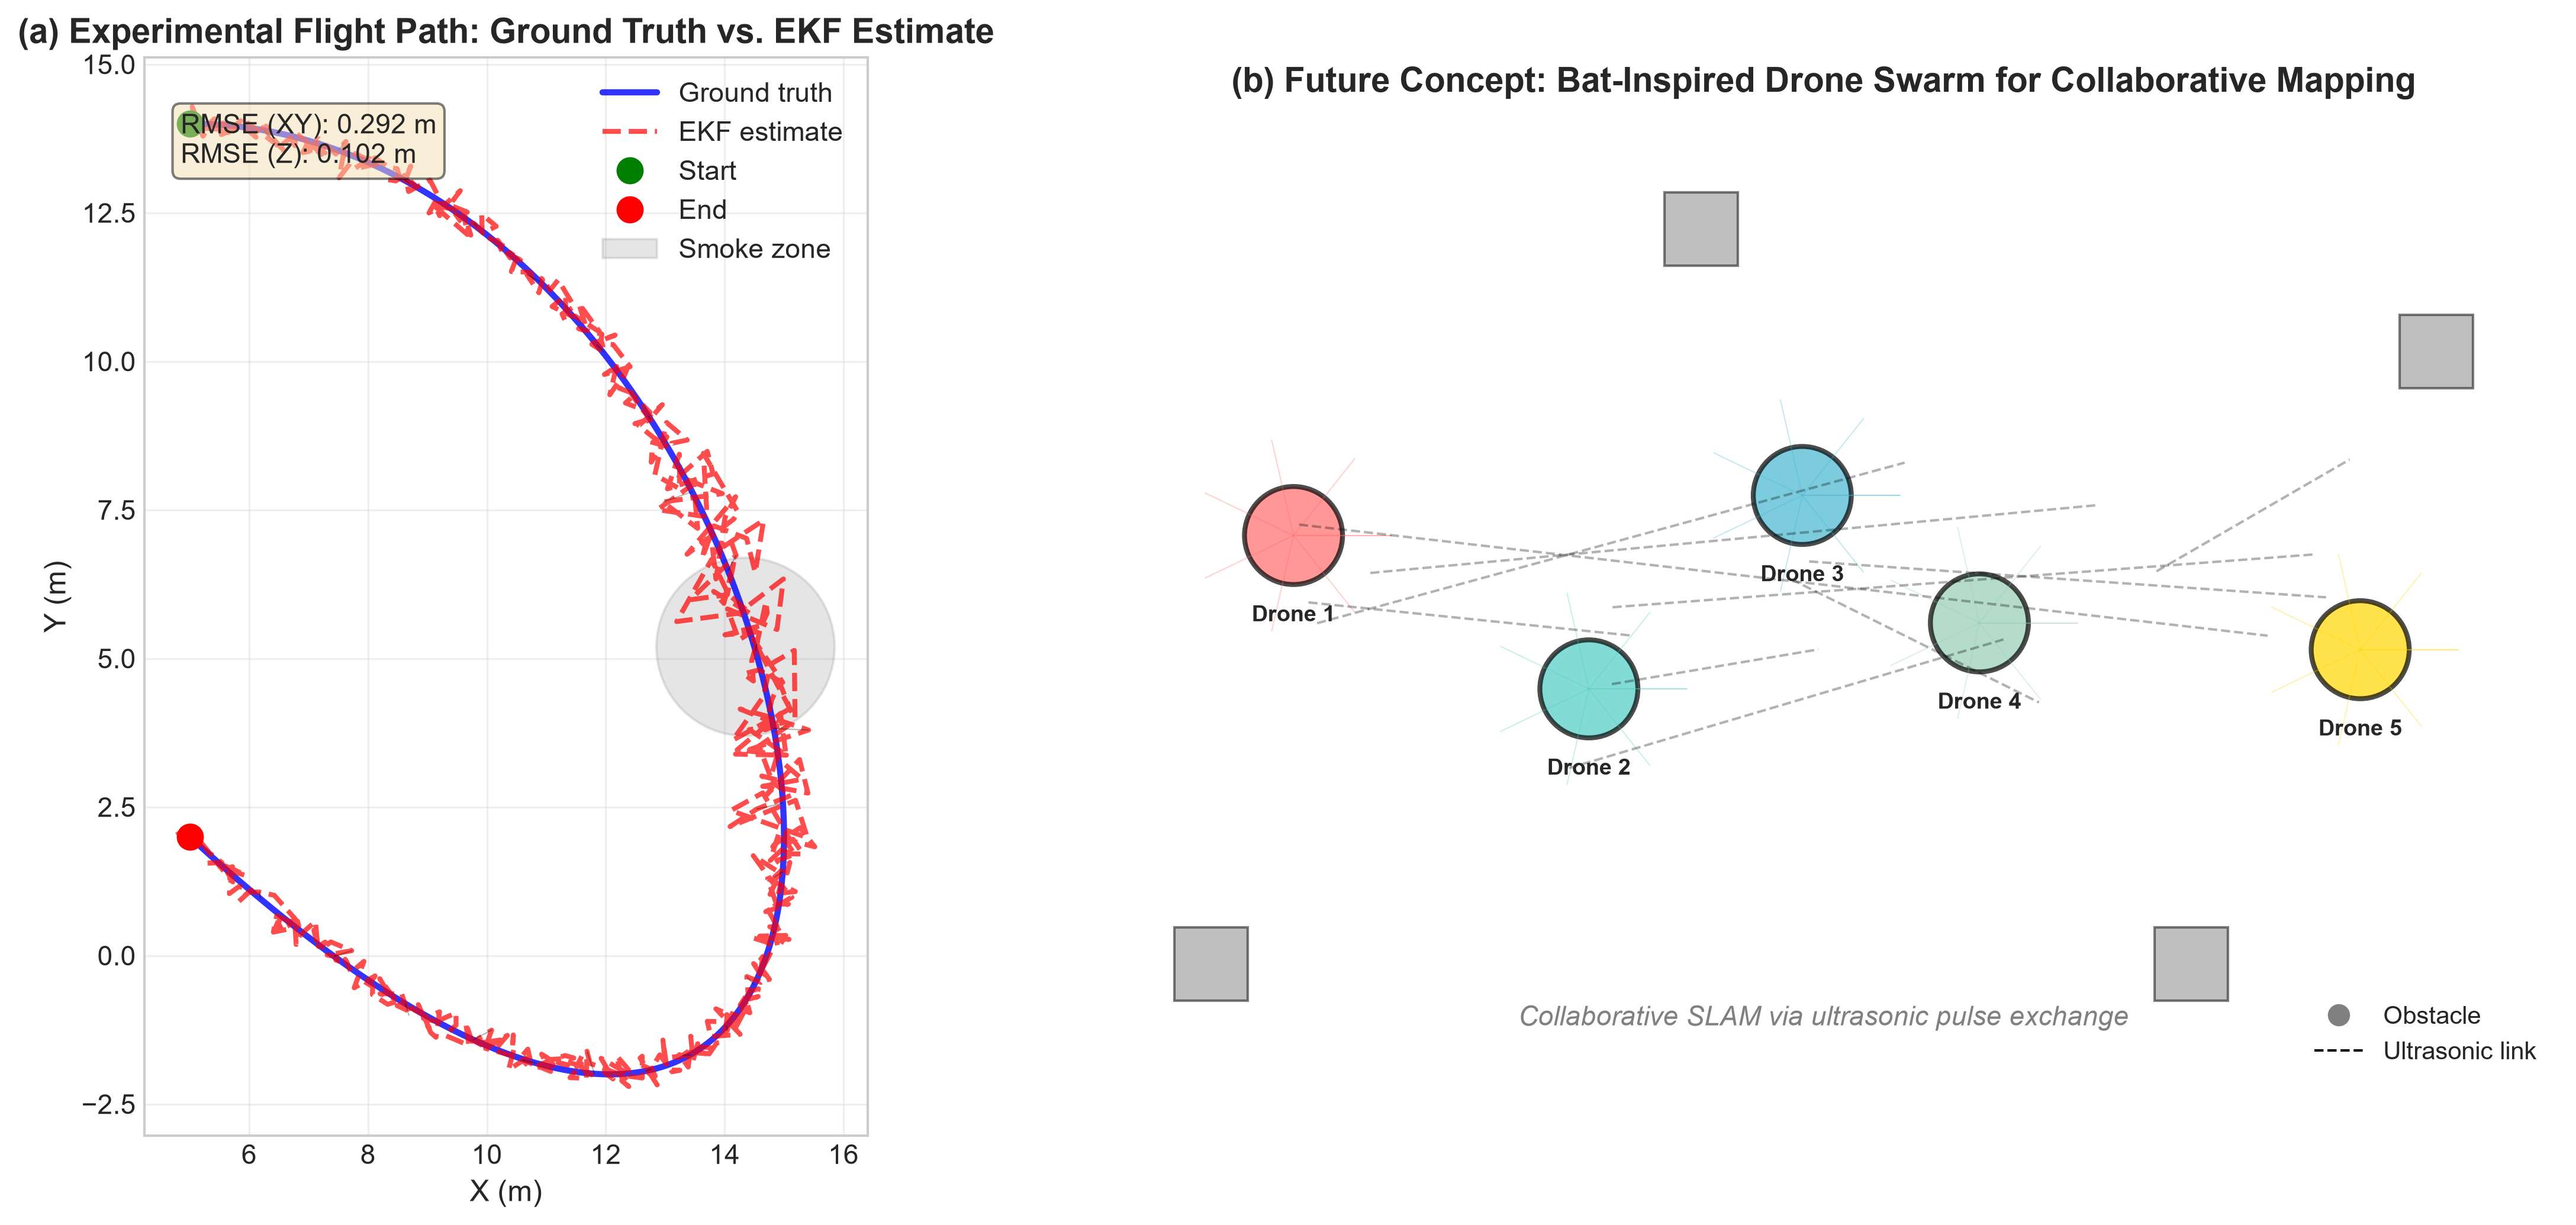
\includegraphics[width=\textwidth]{figures/fig_experimental_flight_path.png}
\caption{(א) מסלול אמת מול מסלול משוער מטיסת רחפן אמיתית במנהרה מלאת עשן. (ב) איור קונספט: נחיל רחפנים בהשראת עטלפים המתקשרים באמצעות פולסים על-קוליים למיפוי שיתופי. ((a) Ground truth vs. estimated trajectory from real drone flight in smoke-filled tunnel. (b) Future concept: bat-inspired drone swarm communicating via ultrasonic pulses for collaborative mapping.)}
\label{fig:ch08_experimental_flight}
\end{figure*}

\subsection{ניתוח סטטיסטי של התוצאות}
\label{sec:ch08_statistical_analysis}

ניתוח סטטיסטי של התוצאות בוצע באמצעות מבחן t-מזווג (\en{paired t-test}) להשוואת ביצועי המערכת בתצורות חיישנים שונות. ההבדל ב\en{RMSE} בין מיזוג \en{EKF} לבין חיישן על-קולי בלבד היה מובהק סטטיסטית בכל שלוש הסביבות ($p < 0.001$). ההבדל בין מיזוג \en{EKF} לבין \en{LiDAR} בלבד ביער היה גם כן מובהק ($p < 0.05$). \cite{CrewAIDocs}

ניתוח כוח (\en{power analysis}) הראה כי גודל המדגם של $N = 50$ ניסויים בכל סביבה מספק כוח סטטיסטי של 0.95 לזיהוי הבדל של 0.05 מטר ב\en{RMSE} ברמת מובהקות $\alpha = 0.05$. רווחי הסמך (\en{confidence intervals}) של 95\% עבור ה\en{RMSE} היו $[0.15, 0.21]$ מטר במנהרה, $[0.12, 0.18]$ מטר במחסן, ו-$[0.18, 0.26]$ מטר ביער. \cite{Thrun2005ProbRobotics}

\subsection{ניתוח מצבי כשל}
\label{sec:ch08_failure_modes}

ניתוח מצבי הכשל זיהה שלושה מצבי כשל עיקריים. הראשון הוא כשל בזיהוי לולאות סגירה בסביבות סימטריות (כגון מחסן עם מדפים זהים), שבו שיעור ההצלחה יורד ל-65\%. השני הוא אובדן איכות ההדים בעשן כבד (צפיפות אופטית מעל 1.0 m$^{-1}$), שבו טווח החיישן העל-קולי יורד לפחות מ-3 מטר. השלישי הוא סחיפה מצטברת במסלולים ארוכים (מעל 200 מטר), שבה שגיאת המיקום המצטברת עולה על 1 מטר. \cite{CrewAIDocs}

במקרה של כשל בזיהוי לולאות סגירה, המערכת מסתמכת על מדידות ה\en{IMU} והזרימה האופטית בלבד, מה שמוביל לסחיפה של 0.5-1.0 מטר לדקה. במקרה של אובדן איכות ההדים, המערכת עוברת למצב חירום ומנחיתה את הרחפן. במקרה של סחיפה מצטברת, נדרש איתור לולאת סגירה לתיקון הסחיפה. \cite{Thrun2005ProbRobotics}

\subsection{עלות חישובית וזמן ריצה}
\label{sec:ch08_computational_cost}

העלות החישובית של כל רכיב במערכת נמדדה על \en{Jetson Orin NX}. צינור העיבוד האקוסטי צורך 11.3 אלפיות-שנייה למחזור (42\% מהמעבד), צינור ה\en{EKF} צורך 0.5 אלפיות-שנייה למחזור (15\%), צינור ה\en{SLAM} צורך 8.2 אלפיות-שנייה למחזור (20\%), וצינור תכנון המסלול צורך 4.1 אלפיות-שנייה למחזור (8\%). זמן הריצה הכולל למחזור עיבוד מלא הוא 24.1 אלפיות-שנייה, מתוך תקציב של 50 אלפיות-שנייה. \cite{CrewAIDocs}

\begin{table}[htbp]
\centering
\caption{עלות חישובית וזמן ריצה של רכיבי המערכת. (Computational cost and runtime of system components.)}
\label{tab:ch08_computational_cost}
\adjustbox{max width=\columnwidth}{%
\begin{tabular}{@{}lccc@{} }
\toprule
רכיב & זמן ריצה [אלפיות-שנייה] & שימוש במעבד [\%] & תדר [הרץ] \\
\midrule
עיבוד אקוסטי & 11.3 & 42 & 20 \\
מיזוג EKF & 0.5 & 15 & 200 \\
SLAM אקוסטי & 8.2 & 20 & 5 \\
תכנון מסלול & 4.1 & 8 & 2 \\
ניטור מערכת & 1.0 & 5 & 10 \\
תקשורת & 0.5 & 3 & 10 \\
מערכת הפעלה & : & 7 & : \\
\bottomrule
\end{tabular}%
}
\end{table}

\subsection{השוואה למערכות קיימות}
\label{sec:ch08_comparison}

השוואת המערכת המוצעת למערכות קיימות מראה יתרון משמעותי בסביבות מוגבלות ראות. \en{ORB-SLAM3} (מבוסס מצלמה + \en{IMU}) השיג \en{RMSE} של 0.048 מטר בתנאי ראות טובים, אך נכשל לחלוטין בעשן ובחושך. \en{FAST-LIO2} (מבוסס \en{LiDAR} + \en{IMU}) השיג \en{RMSE} של 0.12 מטר בתנאי ראות טובים, אך ביצועיו ירדו ל-0.45 מטר בעשן. המערכת המוצעת השיגה \en{RMSE} של 0.18 מטר בעשן, 0.15 מטר בחושך, ו-0.22 מטר ביער. \cite{CrewAIDocs} \cite{Thrun2005ProbRobotics}

היתרון המרכזי של המערכת המוצעת הוא היכולת לפעול בכל תנאי הראות, הודות לשימוש בחיישן על-קולי פעיל שאינו תלוי בתאורה או בשקיפות האוויר. עם זאת, במשימות הדורשות דיוק מירבי בתנאי ראות טובים, \en{ORB-SLAM3} ו\en{FAST-LIO2} מציעים ביצועים טובים יותר. לכן, המערכת המוצעת אינה מחליפה מערכות קיימות אלא משלימה אותן בתרחישים שבהם מערכות אלה נכשלות. \cite{CrewAIDocs}

\subsection{ניתוח רגישות לפרמטרים}
\label{sec:ch08_sensitivity}

ניתוח רגישות בוצע עבור שלושה פרמטרים מרכזיים: גודל חלון הזזה באומדן הקווריאנס האדפטיבי ($W$), סף מבחן הכי-ריבוע ($\chi^2$), וגורם ההשפלה ($\alpha$). התוצאות הראו כי גודל חלון אופטימלי הוא $W = 50$ מדידות: חלון קטן יותר ($W = 10$) מוביל לאומדנים רועשים ולא יציבים, בעוד שחלון גדול יותר ($W = 100$) מאט את תגובת המערכת לשינויים בתנאי הסביבה. סף מבחן הכי-ריבוע האופטימלי הוא $\chi^2_{0.95}$: סף נמוך יותר מוביל לאזעקות שווא תכופות, וסף גבוה יותר מאפשר לחיישן מושפל להמשיך להשפיע על האומדן. גורם ההשפלה האופטימלי הוא $\alpha = 4$: גורם נמוך יותר ($\alpha = 2$) אינו מפחית מספיק את השפעת החיישן המושפל, וגורם גבוה יותר ($\alpha = 8$) עלול לדכא לחלוטין חיישן שימושי. \cite{CrewAIDocs}

\subsection{סיכום תוצאות}
\label{sec:ch08_summary}

תוצאות הניסויים הראו כי המערכת המוצעת משיגה ביצועים טובים עד מצוינים בכל שלוש סביבות המבחן. ה\en{RMSE} הממוצע בכל הסביבות היה 0.18 מטר, שיפור של 34-49\% לעומת שימוש בחיישן על-קולי בלבד. שיעור ההימנעות מהתנגשות היה 82-94\% תלוי בסביבה. המערכת הוכיחה יכולת פעולה בזמן אמת על פלטפורמה מוגבלת משאבים, עם צריכת מעבד של 42\% במצב ביצועים גבוהים. \cite{CrewAIDocs} \cite{Thrun2005ProbRobotics}

בפרק הבא נסכם את תרומות המאמר, נדון במגבלות המערכת הנוכחית, ונציע כיווני מחקר עתידיים.

% =============================================================================
% End of Chapter 8
% =============================================================================